
\chapter{Configuration Assumptions}

For this study a simple fixed-wing tractor configuration was chosen as the baseline for both architectures. 
Common characteristics between the gas and solar models include a constant tapered wing and a conventional tail with a single tail boom extending from the wing.  
The gas powered aircraft has a fuselage to hold all of the fuel required for the mission.  
The solar-electric powered aircraft holds the batteries in the wings.  
The solar cells for the solar-electric aircraft are placed along the wing and possibly on the horizontal tail.  
A simple diagram of each vehicle is shown in Figure~\ref{f:simpleaircraft} with their corresponding weight breakdowns in Figure~\ref{f:wbreak}.
The configuration is assumed to be static for this study.

\begin{figure}[h!]
	\begin{center}
	\includegraphics[width=1.0\textwidth,natwidth=447,natheight=265]{simpleaircraft.eps}
    \caption{Blue and red are specific to the solar-electric and gas architectures respectively.  Black are shared characteristics.}
	\label{f:simpleaircraft}
	\end{center}
\end{figure}

\begin{figure}[h!]
	\begin{center}
	\includegraphics[width=1.0\textwidth,natwidth=378,natheight=335]{wbreak.eps}
   \caption{Representative weight breakdown of both aircraft optimization models.}
	\label{f:wbreak}
	\end{center}
\end{figure}
